\documentclass [12pt]{article}
\usepackage{fancyhdr}
\usepackage[utf8]{inputenc}
\usepackage[english]{babel}
\usepackage{gensymb}
\usepackage{amsmath,amssymb,amsfonts}
\usepackage{algorithmic}
\usepackage{graphicx}
\usepackage{textcomp}
\usepackage[table]{xcolor}
\usepackage{siunitx}
\usepackage{indentfirst}
\usepackage[margin=2.5cm]{geometry}
\usepackage{float}
\usepackage{hyperref}
\usepackage[UKenglish]{datetime}
\usepackage{setspace}
\usepackage{hhline}
\usepackage{lastpage}
\usepackage[numbers]{natbib}
\usepackage[acronym]{glossaries}
\usepackage{listings}
\usepackage{color}
\usepackage{booktabs}% http://ctan.org/pkg/booktabs
\newcommand{\tabitem}{~~\llap{\textbullet}~~}
\usepackage{subfigure}

\usepackage{helvet}
\renewcommand{\familydefault}{\sfdefault}

\definecolor{customgreen}{rgb}{0,0.6,0}
\definecolor{customgray}{rgb}{0.5,0.5,0.5}
\definecolor{custommauve}{rgb}{0.6,0,0.8}

\graphicspath{{images/}}

\hypersetup
{
    colorlinks=true,
    linkcolor=black,
    urlcolor=blue,
    citecolor=black,
}

\doublespacing

\title{Project Execution Plan}
\author{Daniel Cole, Jack Pendlebury, Noah Harvey, Luke Waller}
\date{\today}

\begin{document}

\begin{titlepage}
    \begin{center}
        \vspace*{1cm}

        {\Huge \textbf{Project Execution Plan}}

        \vspace{1.5cm}

        \textbf{Daniel Cole, Jack Pendlebury, Noah Harvey, Luke Waller}

        \today

        \vfill

        Project Execution Plan presented for the HEVCS Master project.

        \vspace{0.8cm}

        
\includegraphics[width=0.4\textwidth]{UOP_Logo.png}

    \end{center}
\end{titlepage}

\newpage
\fancyfoot[R]{Page \thepage \hspace{1pt} of \pageref{LastPage}}
\setcounter{page}{1}
\pagenumbering{arabic}
\tableofcontents
\newpage

\newpage
\section{Project Overview}\label{sec:section_1}
\subsection{Business Justification}\label{sec:business_justification}
%%%%reference in here
The HEVCS aims to overcome challenges related to the lack of EV charging infrastructure in a world where the number of EVs on the road is growing at an increased rate every year. Solutions to incorporate EV charging points into our homes, carparks, and workplaces will not overcome the barriers created by the way in which pre-existing infrastructure has been designed. Over 60\% of UK homes do not have access to a garage or a driveway in which an EV charging port could be safely installed \cite{60_no_parkers}, stripping away a large proportion of the population's ability to own an electric powered vehicle.

\subsection{Sirmon Industries Sponsorship}\label{sec:sponsorship}
Sirmon Industries are a design consulting firm with a wide range of experience in many engineering disciplines. They have conducted work across many sectors such as film industry props, special effects for the entertainment industry, passenger information systems, outdoor display systems, as well as home domestic equipment and high-end industrial products. The company provide a bespoke service covering all stages of the development process. This includes the planning phases, project direction, and project scope. They offer a full suite of software design, in addition to their hardware and mechanical engineering capabilities, including PCB design and embedded systems. Their online presence and portfolio documents rapid prototyping and development for a wide range of products, providing inspiration to those who share the same enthusiasm for innovation in their fields.

The sponsorship opportunity was a result of Sirmon identifying a problem that is becoming increasingly prevalent in day-to-day life and seeking university students to create a prototype for their master’s project.

\subsection{European Social Fund Grant}\label{sec:esf_grant}
The University of Plymouth receives grants from the European Social Fund (ESF) to enhance students’ learning and development of skills. The ESF aids students to overcome the barriers associated with accepting opportunities by donating the necessary financial funding and sourcing additional sponsorship from external companies, such as Sirmon Industries. In return, the organisation request timesheets detailing the time spent on each project related activity. These are accompanied by Smart Specialisation Curriculum and Engagement reports with overviews of the project, group members and methodology.
After securing the grant, an academic and technical support assistance was assigned to the group. Jo Byrne’s role is defined in greater detail in section \ref{sec:Leadership_and_Team_Organisation}, as the team must provide regular updates on work progression and collaboration with Sirmon Industries.


\subsection{Design Requirements}\label{sec:design_requirements}
The scope of the project has been defined by the following requirements: \\

1.	The platform must abide by class 2 mobility scooter legislation and the respective highway regulations to be road legal. \\
2.	The platform must be able to navigate the home, roads and pavements and the relevant obstacles such as kerbs and a maximum of three steps while transporting the payload from the user’s home to their car. \\
3.	The platform must be always controlled by the user via a tethered connection to move. Upon disconnection, the device enters an immobilised state. \\
4.	The robot must be capable of acknowledging hazards, such as too steep a slope, too many steps and obstructions. In these cases, the robot must refuse to tackle such obstacles and override the user’s inputs. \\
5.	The platform must be stored safely within the docking station that minimises the space in which it occupies whilst it charges the EV battery. \\
6.	The platform must be able to drive underneath EV’s with a ground clearance of 155mm and above and lock itself securely to the vehicle. \\
7.	The platform will not attempt to traverse inclines/declines greater than 20 degrees. \\

\subsection{Deliverables}\label{sec:deliverables}

\begin{table}[H]
    \centering
    \setlength{\arrayrulewidth}{1.5pt}
    \begin{tabular}{|c| p{0.8\textwidth}|}
    \hline
    \cellcolor{gray!40}Deliverable & \cellcolor{gray!40}Details \\
    \hline
    1 & The creation of a wheeled platform capable of supporting a 100KG payload. \\
    \hline
    2 & A wired, tethered controller for the platform, capable of controlling all functions.
    The connector will be of a magnetic breakaway design, immobilising the motors if the link is broken. \\
    \hline
    3 & The platform’s total height must be less than 150mm. \\
    \hline
    4 & The platform will be able to move in all four cardinal directions via use of the mecanum wheels, to ‘strafe’ underneath parked vehicles. \\
    \hline
    5 & The platform will be able to drive, and navigate, upon a maximum of a 20-degree inclination. \\
    \hline
    6 & The platform will be able to navigate a maximum of 3 standard sized steps, as well as kerbs of a reasonable height. \\
    \hline
    7 & The platform will make use of sensors to assist the user in navigating around obstacles. \\
    \hline
    8 & The platform will comply with all relevant ‘invalid carriage’ legislation, to allow it to be used on the pavements without penalty. \\
    \hline
    9 & An android app will be used to gather telemetry from the platform and be used to lock and unlock the motors. \\
    \hline
    \end{tabular}
    \caption{Deliverables}
    \label{table:deliverables}
\end{table}

\subsection{Milestones}\label{sec:milestones}

\subsubsection{Milestone 1 - Static Motor Test Platform}
A static motor test platform, using the drive motors, ESCs, and desired gearing system, controlled using a static control panel. This platform will be used to demonstrate operation of the motors and ESCs, as well as to measure the functional torque of the drive system.

\subsubsection{Milestone 2 - Handheld Controller, Breakaway Connector, and Immobiliser}
The platform in milestone one will be augmented with the handheld controller, complete with magnetic breakaway connector. This will be used to test controller technologies, and safety features. Any changes to the safety cut-off will be tested on this platform first.

\subsubsection{Milestone 3 - Mobile Aluminium Chassis}
The proven technologies from milestone two will be added to a mobile aluminium extrusion chassis. This will be used to test internal component layouts and mecanum wheel functionality. The platform must be able to drive in all directions on a flat surface.

\subsubsection{Milestone 4 - Mobile Weight Bearing Chassis}
With the internal layout and motor control functionality demonstrated, the aluminium chassis will be replaced with one that can support the full battery payload weight, without compromising functionality.

\subsubsection{Milestone 5 - Platform with Object Avoidance}
Milestone four’s upgraded chassis will have the object sensing and ranging user assistance features added. This milestone will not be passed until all sensors are functional, and the platform can correctly sense impending collisions and drops beyond the specified three step limit.

\subsubsection{Milestone 6 - Platform with Step/Kerb Navigation}
The object avoidance features in the prior milestone will be used to facilitate step climbing and descent. The system will use the milestone 5 sensor array to prevent it from descending inclines beyond the three-step limit for safety reasons.

\subsection{Key Constituent Parts}\label{sec:key_constituent_parts}

\begin{table}[H]
    \centering
    \setlength{\arrayrulewidth}{1.5pt}
    \begin{tabular}{|c| p{0.6\textwidth}|}
    \hline
    \cellcolor{gray!40}Key Component & \cellcolor{gray!40}Description \\
    \hline
    Load Bearing Chassis & A rectangular based chassis containing the control systems, motors, drivetrain, sensor mounting points, and space for the payload. Internal systems will be attached using a modular rail system to facilitate easy replacement. The chassis must be no taller than 150mm.\\
    \hline
    Controller & A handheld controller, connected via a breakaway connector, that allows the user to control the functions of the system. This will allow the user to drive the platform using two analogue sticks, one for each wheel. The user will be alerted should any of the sensor assemblies detect an obstacle, or if the ranging detects that a descent is further than three steps. An LCD screen will report the system status to the user. Will either be battery powered or powered through the tethered connector.\\
    \hline
    Sensor Assemblies & Adjustable, modular sensor assemblies for mounting on the chassis. Their aspect and bearing can be adjusted to provide the desired coverage. While each assembly may have different sensors within it, each mounting bracket will be the same, so sensors can be repositioned at will.\\
    \hline
    Controller Connection cable & The controller connection cable will make use of a magnetic breakaway feature. Should the platform be in a position where it begins to run away from the user, the force will disconnect the controller. This will prevent the user from being pulled over and trigger the safety locks within the motor assembly, preventing further runaway movement of the platform. This connector will be 10 pins, with a central ground. \\
    \hline
    Central Control Unit & The central control unit will be mounted using modular rails described above and will contain the microcontroller as well as all the necessary interfaces to communicate with the sensor assembly suite and motor drivers. \\
    \hline
    Motor Assembly and Drivetrain & The motors, pulley drivetrain, and ESC motor controllers, will be mounted to the chassis. These will be connected to the central control unit with control lines.\\
    \hline
    \end{tabular}
    \caption{Key Constituent Parts}
    \label{table:key_constituent_parts}
\end{table}

\subsection{Predicted Challenges}\label{sec:predicted_challenges}

\subsubsection{Project Requirements}
The stated battery payload capacity of 15kWh minimum places a heavy burden on the chassis. Depending on the specific power cells purchased, the total EV battery payload is expected to fall between 70 and 120 kgs. Given the environmental navigation requirement specified in requirement two, the chassis must be able to withstand this weight in conditions where not all wheels are contacting the ground, or sections of the chassis are unsupported.

While strength is a requirement, it is also equally important to balance strength vs weight. With such a heavy payload, any additional weight is unnecessary strain on the drive system. More weight means more torque needed from the motors, more strength in the wheels, and a more sophisticated obstacle navigation system. The weight is additionally constrained by legislature pertaining to the classification of electrically driven vehicles, and the restrictions therein.

Safety of both the user and other pedestrians is also a significant concern. At the limit of 4 mph (1.8 m/s), a 100KG chassis will have significant kinetic energy, and with the torque required to move such a weight, significant injury could be caused to a pedestrian. Impacts with terrain and obstacles could cause heavy damage to both property and to the platform, with a risk of compromising the battery payload.

The team collected data about car dimensions for EVs being released in 2022 and found that a height requirement of 155mm will allow the HEVCS platform to fit underneath 53\% of vehicles. The data can be found in section \ref{app:Car_Dimensions}. Ensuring that the design is compact enough to fit underneath a vehicle will provide a significant challenge; a focus on compact design methodologies will have to be maintained throughout all related components of the design.


\subsubsection{Sponsorship Challenges}
The team must allocate more time to discuss the project's progress amongst themselves, the supervisors and Sirmon. Sirmon must be involved in each project stage and have time dedicated to discussing and fulfilling the requirements they defined in the scope. In order to keep the meetings concise to increase time efficient, Zoom meetings involve the team giving an overview of the week's output. The necessary documents are emailed to allow Sirmon to read them in their own time.

The technical work completed will be documented in detail using OneNote, in a manner that allows another team member, who did not initially carry out the task, to replicate the work. The critical design ideas and developments will be stored in the form of sketches. This will include anything between rough drawings, wiring diagrams and brainstorms to maintenance tests. The problems that arise will be reported, along with any necessary information of the scenario in which the problem occurred. Then, upon finding a solution, a detailed step by step guide of how this was achieved will also be created. All of which will be made accessible to supervisors and Sirmon.

Additional reports required for the sponsorship must be completed alongside the technical work and course related reports. To complete these reports in an efficient manner, the material they require is summarised by the team at the end of each working week. These summarise are tailored to meeting the criteria of the debriefs provided by the sponsorship team.

\subsubsection{HEVCS Build and Operation}

The platform must be built by those who have signed the risk assessments, and in a safe environment with the necessary safety equipment. The platform must be stored in a secure room, and in a safe manner. Once the system is operational, and driving test are being conducted via the controller, the testing area must be clearly marked, and no members of the public can be present.

The global shortage of electronic components has had and continues to have massive ramifications for any project. With the shortage of semiconductors, many microcontrollers have long lead times, consequently ordering microcontrollers for this project would not be feasible. The team will be using Nucleo-F429ZI boards that they already own to help alleviate the supply chain issue on microcontrollers. Other factors, such as global warming and the Russian invasion of Ukraine, have also supplemented supply chain issues. Global warming has cause draughts, fires, and flooding all over the globe which has affected suppliers' ability to produce the raw materials for manufacturing components. Russia's invasion of Ukraine has impacted the supply of Neon gas, which is a commonly used when laser cutting, causing manufacturers to struggle with the demand for their products \cite{Supply_Chain}. Due to these factors, the team may struggle to order components for the HEVCS platform within the time scale of the project. The inflated prices will make procuring the components within the budget more challenging.

\section{Legal Requirements}
\subsection{Legal Restrictions of Use}
The platform will be made to abide class 2 invalid carriage legislation \cite{Invalid_Legislation}, restricting it to a maximum speed of 4mph. It will be compact and as lightweight as possible and compact to accommodate to manoeuvring around homes. Class 2 invalid carriages do not need to be registered with the DVLA.

\subsection{Relevant Legislation}
\subsubsection{Highway Regulations}
The platform must be built to follow the legislation for a class 2 invalid carriage, detailed in the Use of Invalid Carriages \cite{Invalid_Legislation} on Highways Regulations. This device must be mechanically propelled and incapable of exceeding 4mph. The maximum unladen weight of the platform is 113.4kg, where the definition of 'unladen carriage' is inclusive of the weight of water, fuel, power equipment for the platform itself and the propulsion equipment. It does not include the weight of any other load, including the weight of the EV batteries that the robot will transport.

The maximum dimensions of the platform are a product of the hallway, doors, and entrance dimensions within the home, as well as the distance between wheels on the most common EVs. With a maximum height of 155mm, the device would be able to successfully transport a payload underneath 53\% of the most common EVs. As class 2 mobility scooters are made to be used indoors, their dimensions determined the maximum length and width is 1000mm and 500mm, respectively.

\subsubsection{Road Traffic Act 1972}
Other requirements include the functionality of a lights as a motor vehicle would under the Road Traffic Act 1972 \cite{Road_Traffic}. It must also be capable of breaking within a reasonable distance, in all conditions, and remaining stationary on a slope of gradient 1m over a horizontal distance of 5m. The braking system required to hold the platform stationary cannot rely on the limiting of electrical current, hydraulic or pneumatic devices.


\section{Project Management}\label{sec:project_management}

\subsection{Project Management Analysis}\label{sec:project_management_analysis}
The first step in the process of selecting a project management method was defining what core values are important to the team and the customer. A meeting was held to discuss individual team members opinions to highlight the common methods, procedures, and techniques that the chosen methodology should possess. This ensured that the project management techniques used were catered to the research problem and focused on accommodating to the project’s deliverables.

Overall, the team wanted to define roles and split the tasking to suit the individual’s strengths and skills. This then expanded to involve a requirement for the tasks to be justified, return beneficial outputs and be a good use of time and resources. With the milestones outlined alongside the customer, and incorporating the team’s previous experiences, the larger and more complex tasks were highlighted. Stakeholders expressed a concern that the team acknowledge, and began to break the tasks down into smaller, more achievable goals.

Whilst researching how to overcome complex obstacles, the agile methodology was discussed for its ability to adapt to challenges and accommodate to sudden change of approach. On the contrary, the waterfall methodology raised multiple concerns which the team felt would be detrimental to the project’s outputs. To select a suitable approach, various models were analysed in more depth, along with considerations into the IET’s encouraged methodology training and ISO series 21502 from the International Organisation for Standardization.

The project management analysis meeting took another approach that featured outlining what processes or situations would have a negative impact on the project. This raised the common issues that occur from poor communication, organisation, and file management, but also the prevalent challenge of purchasing parts from within the UK when facing stock shortages and extended wait times. The team then discussed altering the project plan to focus on completing health and safety documents that would allow for component and part orders to be placed well in advance of the build phase. The GANTT chart was additionally altered to include shorter meetings with the team to discuss purchasing components needed down the line, ready for the next build/design iteration. Again, agile methodology would greatly mitigate the risk of a delay in obtaining parts, and therefore the progress of the project, by altering the tasks orders.

\subsection{Agile Methodology}\label{sec:agile}
The methodology defines a set of principles, tools and techniques that are used to plan, execute, and manage the project. With a team consisting of four members with varying schedules, an agile methodology would accommodate self-organisation for all individuals. The project planning itself, along with the management of the tasks being defined, has adaptivity as a key paradigm. This enables evolutionary development which facilitates prompt delivery of progressive achievements that are not necessarily in order, unlike waterfall project management. By using such a responsive methodology, with regular review, the team can adjust tasking and focus on continuous improvement in all aspects.

Within the agile methodology consists of multiple values, the first being that your team is your most valuable resource. All the processes involved only work if the team members are performing well. By focusing on how the team communicates, shares ideas and support one another, the quality of the output is also increased. Regular engagement from the customer, Sirmon Industries, enforced the importance of collaboration and feedback. This benefited the project's evolution from idea to final product while creating a collaborative space to communicate openly.

\subsection{Waterfall Methodology}\label{sec:waterfall}
The waterfall approach to project management is based on linear progression, from planning to execution. Tasking is carried out sequentially, with design, development and testing happening in turn \cite{Waterfall_Meth}. It requires each stage to be completed before the next phase begins, which does have its advantages. Whilst working on one phase, there is the guarantee of easier project management and the potential to complete tasks efficiently. On the other hand, the project’s progress can be halted due to delays within a single phases task completion.

This method relies heavily on the project requirements being stated, and made permanent, at the start of the planning phase. The team and customer discussed previous experiences of carrying out similar projects and shared the concern that the requirements and the order of tasking cannot be permanently fixed.  Implementation of software and new components for testing does not always go to plan, or resemble a smooth and linear process, and challenges can arise before the deployment phase is reached. The methodology used for this project must accommodate the development of various aspects simultaneously, with the ability to adapt or adjust the tasking as the project advances.



\subsection{Methodology Analysis}\label{sec:methodology_analysis}
Each team member rated the various principles of project management by their importance. This information has been documented in the methodology research spreadsheet, along with a scoring system for each approaches performance to the respective principle. The table below shows the personal importance ratings, and the average score of each principle.

\begin{figure}[h]
    \centering
    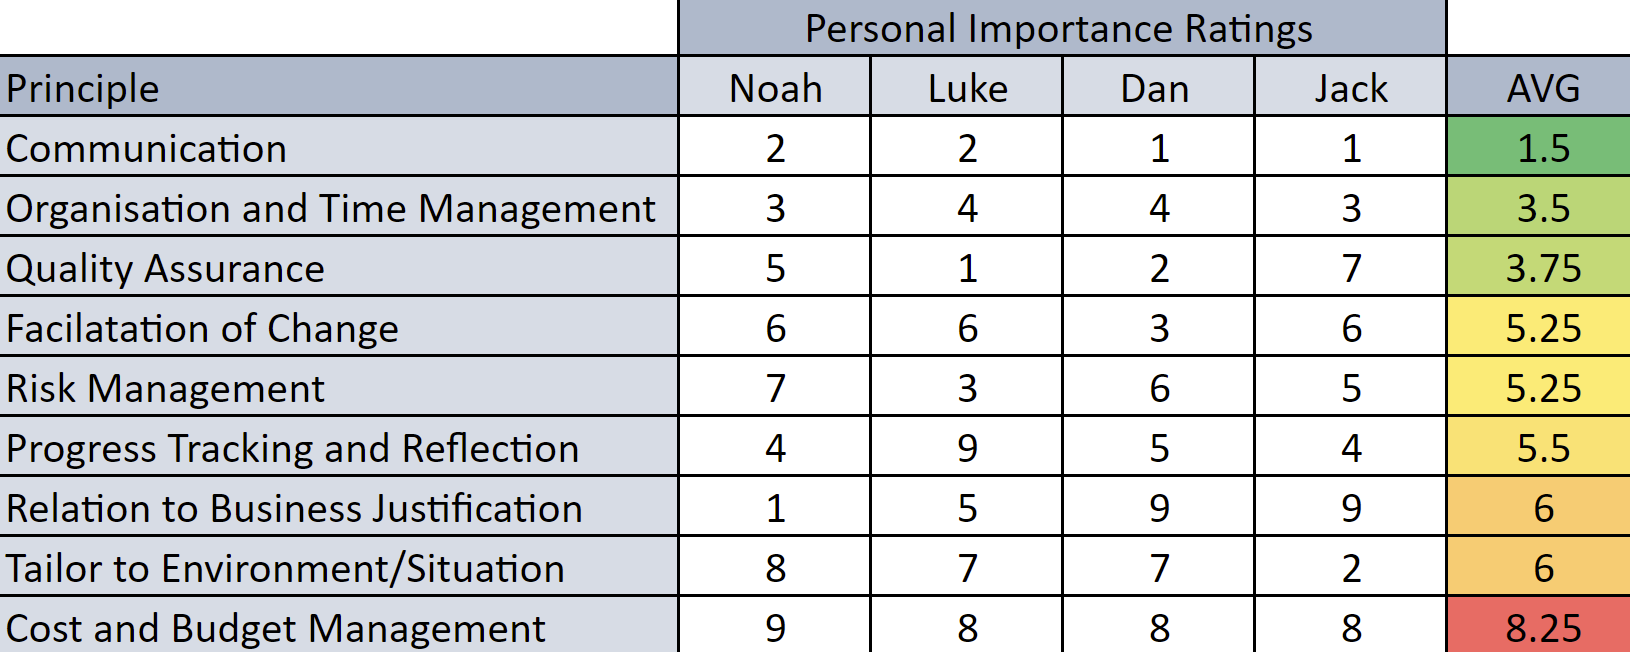
\includegraphics[width = 8cm]{PersonalPrincipleRatings.png}
    \caption{Personal Principle Ratings}
\end{figure}

This exercise highlighted that the team valued communication, quality assurance, and organisation and time management. As the project develops, the skills that the team members have obtained from previous experience, and the importance of the principles to them as individuals, will have a direct impact on the development of the project.

The table can be used to assign tasks based on the differences between the individual's opinions, assigning the principle's related responsibilities to the members who rated them highest. For example, Jack felt that tailoring the project methodology to the environment and scenario was of high importance. The rest of the team did not share this opinion, so when discussing the ways in which the methodology could be adapted for this scenario, Jack was able to lead the conversation and bring a different skill set. Further tasking allocations are discussed in the roles and responsibilities section.

This activity also outlined the principles that obtained the lowest levels of importance, provoking reflective discussions between team members. The first outcome that arose from this discovery was the steps the team could make to prevent these. The GANTT chart and meeting minutes template will include scheduled discussions specifically for discussing business justification and budget management.

\subsection{Chosen and Adapted Methodology}\label{sec:chosen_methodology}
While researching the IET’s suggestions for project methodology, a course that detailed seven principles, themes and processes which combined to create the \cite{PRINCE2} agile and process-based approach to project management. All the key attributes detailed in the overview of this widely adapted training course were used to outline the team's approach to this project. This also provided a checklist in which the various methodologies could be scored against to adapt specific elements to suit this project. Each principle, theme and process has been discussed individually to apply the most suitable methodology to each. Adaptions to the principles have been made according to wish methodology's approach the team gave a higher score in the methodology analysis table below.

\begin{figure}[h]
    \centering
    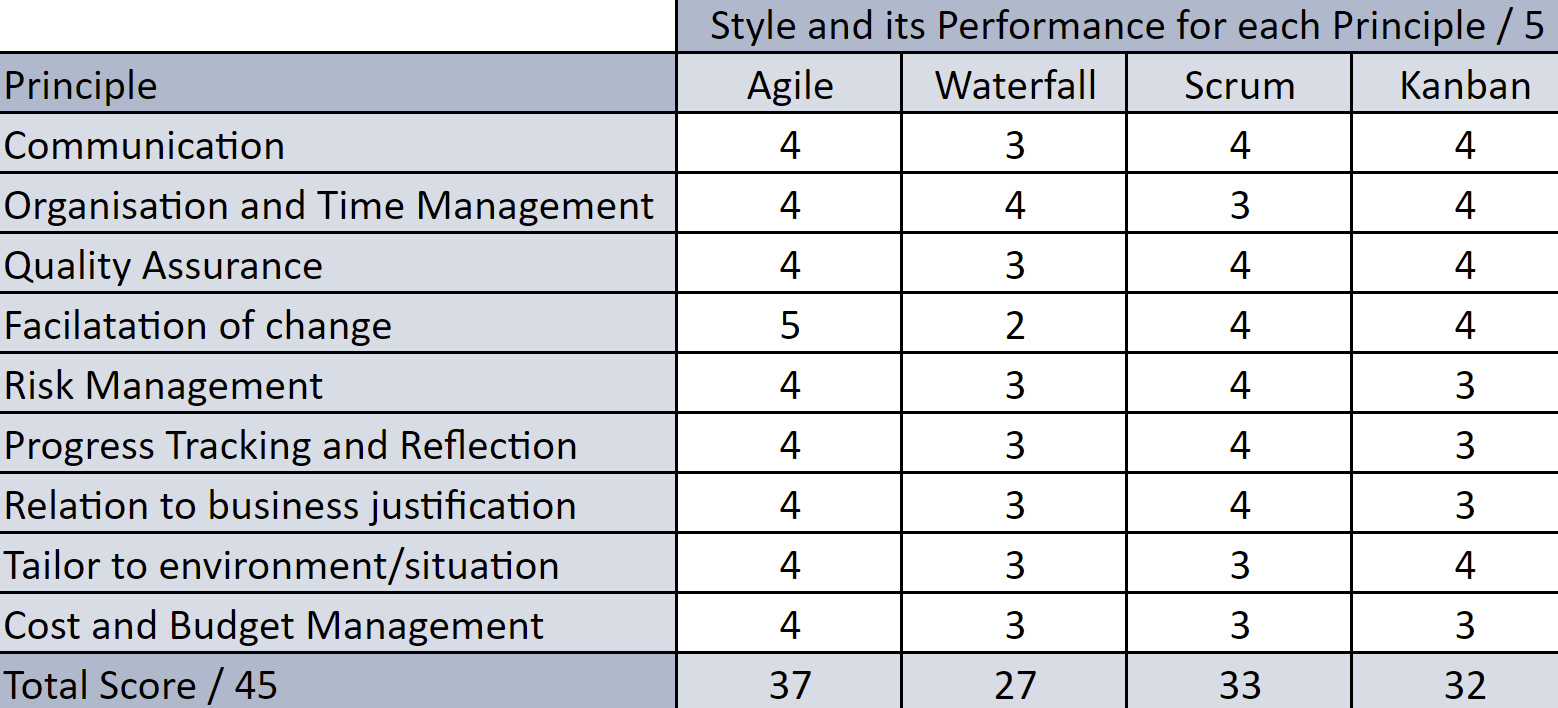
\includegraphics[width = 8cm]{PrincipleMethodologyRating.png}
    \caption{Principle Methodology Ratings}
\end{figure}

\subsection{PRINCE2: The 7 Principles}\label{sec:7_principles}

\textbf{Business Justification} \\
Continued business justification. There is a requirement for a product such as the HEVCS, and therefore there is a strong business justification. The project must continue to incorporate the important features that would return an investment for the time and resources.

\textbf{Learning from Experience} \\
Learn from experience. The team consist of members with previous experience of carrying out projects from start to finish, alongside the customer who would be described as a ‘serial inventor’. These experiences keep the goals realistic, achievable and provide valuable lessons learned. During this project a log with be kept, documenting what individual team members have learned, from both positive and negative experiences.

\textbf{Defining Roles and Responsibilities} \\
Define roles and responsibilities. The team have written personal statements that detail their skills, previous jobs and general interests that relate to the project. A discussion was held to define the role of all members and their tasking as the team recognise the importance of utilising an individual’s assets. The team are made aware of their tasks in meetings through action assignment, by task delegation in the Kanban board and from continuous communication. Each written element has an original author, then a checker to proofread, followed by an overall approval meeting to finalise that element of the project.

\textbf{Managing Stages} \\
Manage by stages refers to breaking down the more challenging elements of the project, as stated in the predicted challenges section of the project overview. Different approaches are taken depending on the task at hand. The team have defined the stages of development for both hardware and software elements of the project.

\textbf{Managing Exceptions}\\
Manage by exception defines the managers input and level of intervention. This project, being sponsored, has various levels of management that require different levels of communication and intervention. This is explained in more detail within the team organisation section.

\textbf{Focus on Products}\\
Focus on the product and what its expected features are. The product requirements have been analysed in the specification document.

\textbf{Tailor to the Environment}\\
Tailor to environment refers to the scalability of the PRINCE2 methodology, allowing projects to alter the principles to suit their needs – well suited to a university project with different requirements from academic and industrial viewpoints.

\subsection{PRINCE2: The 7 Themes}\label{sec:7_themes}
These themes provide a regular reminder of the aims of the project, and the focal outcomes which should be in the forefront of the work carried out. They can often be related to areas of knowledge that the principles must operate within when the methodology is put into practice. Similar to the waterfall method, these themes are decided upon at the start of the project planning and monitored continuously from that point on. The project itself can then be tracked by referring to these themes.

\textbf{Business Case}\\
By referring to the business case, the project can always seek to accomplish the goals it was designed to fulfil.

\textbf{Organisation}\\
Organisation of roles and responsibilities earlier on in the project sets a solid developmental plan from which the team members can begin to produce outcomes. It must be noted that the responsibilities can change in accordance with the project’s developments. For example, if another task has a higher priority but the team member with the most knowledge in that area is ill, another member can step in.

\textbf{Quality}\\
Quality can often be an abstract concept as there are so many elements of the project that must be completed to a certain standard. The written communication and documentation must be of high quality to be understood by stakeholders. Each piece of software requires quality assurance, the hardware must be assembled from good quality products and the product itself must be of good quality. Different people can have different standards when referring to something that is of high quality. The important of discussing these standards and what the team set out to achieve has been discussed in more detail for each principle. Testing schemas will be written for both hardware and software at component level.

\textbf{Planning}\\
Planning refers to the timescale, cost, and targets in the form of milestones for the project. It gives the team a set of goals that can be achieved by breaking down the work into separate tasks. This document, the project execution plan, incorporates the goals and tools for how to achieve them into one single plan.

\textbf{Risk}\\
Risk have been identified, assessed, and had preventive measures put in place to apply a certain degree of control over the project. The various types of risk have been discussed in more detail within the health and safety and commercial risk evaluation.

\textbf{Change}\\
Various elements of the project can be subject to change, but the decisions made in relation to the change must be agreed on by the team and Sirmon. The methodology use must not prevent change but enable it by utilising the most appropriate tools to identify the best alternative.

\textbf{Progress}\\
Progress can be shown by transforming the tasking into outputs that, when illustrated by the GANTT chart, can present an overview of regular achievements. The GANTT chart can be seen in section \ref{app:Gantt_Chart}. It is important to track progress and witness regular developments in the project to plan the next steps accordingly, and with an element of strategical flow. It can also highlight incomplete tasks which are taking longer than expected.

\subsection{PRINCE2: The 7 Processes}\label{sec:7_processes}
The processes define the order in which the project is progressed, and the outcomes that require assessment before starting the next stage. With each process overseen by the team members and presented to Sirmon, the management of tasks responsibility and review development are carried out regularly throughout each stage.

\textbf{Project Start Up}\\
Starting up a project requires answering logistical questions about the project and its purpose. It will detail the tasks in respect to linear milestones that constitute a successful project. It then develops into a plan that demonstrates how a task will be done and who will do it. This if often expanded from the specification of the project and its scope.

\textbf{Initiating a Project}\\
Initiating a project outlines the performance targets and milestones that the project aims to achieve. The team does not have a single project manager, but it does have Sirmon as the customer outlining their requirements. The time, cost and scope are all relative to the university’s project brief and incorporate the thoughts of the project supervisor.

\textbf{Directing a Project}\\
Directing of the project is managed by the team as they define their own direction and boundaries for each milestone. Upon completion of a milestone, the evidence and demonstration are provided to both Sirmon and the project supervisor. It is then up to a discussion to ensure all parties agree.

\textbf{Controlling a Stage}\\
Controlling a stage through creating of smaller tasks, which are assigned to individual members, is not the job of one single group member. Meetings are held to facilitate such decisions, and tasks are delegated according to those who are most suited to the job. Each member has the authority to express their opinion on the way in which a task has been carried out, or the product of the task itself.

\textbf{Managing Product Delivery}\\
Managing product delivery refers to the communication that dictates the acceptance of the next stage of the project, its execution, and final delivery. Although the dates are set out in the GANTT chart, the team felt it was important to communicate with Sirmon when starting new tasks. This allows the team to being the task with all the relevant information from all parties and finalise exactly what the proposed outcome should be.

\textbf{Managing Stage Boundaries}\\
Managing stage boundaries would usually require the board to review the tasking and outcome to determine whether the project is to advance further. For this project, it involves a review of the outcomes from a section of the tasking being completed. Scheduling reviews between stages allows the wider team to discuss lesson learned and how the management of the project could be improved.

\textbf{Closing a Project}\\
Closing a project includes an evaluation of the product against the initial business case. If the project is to be developed further, the next actions are also identified. If possible, further testing and operational maintenance should be carried out before customers have access to the product.

\section{Critical Path}\label{sec:critical_path}

\subsection{Stages of Development}\label{sec:stages_of_development}
The stages of development are written in accordance with the project milestones, but multiple stages can operate at the same time. The details regarding the flow of stages are in the Gantt chart in appendix \ref{app:Gantt_Chart}. In this section, each stage's boundaries and results indicative of completion are defined.

The bill of materials are listed in a separate document.

\subsubsection{Stage 1}

Duration: 1 week

\textbf{Motor Testing}\\
This is to ensure that the motors are functioning as they should and operating within the parameters set by the software and ESC. 3D printed brackets will secure the motors during the testing and development phase. The team will carry out torque, speed, braking and immobilisation tests. The testing software will be written for a nucleo board. Programmable routines will be used to run the various tests.

Only upon completion of these tests will the motors enter the next stage of development.

\textbf{Results Indicative of Successfully Completed Stage}\\
1.	A reusable motor testing platform
2.	The motors operate as expected, having passed control tests
3.	The motors can achieve the speed controls set by the controller
4.	The motor speed is limited 4mph
5.	When the controller is not connected, the motors are immobilised

\subsubsection{Stage 2}

Duration: 1 week

\textbf{Controller Design}\\
Designing a controller that can operate the motors, from breadboard to PCB design. Safety features will be testeding to ensure that the controller inputs remain restricted by system overrides values. For example, full throttle does not drive the motors at a speed above 4mph. Additionally, the breakaway cable will be designed and implemented.

\begin{figure}[h]
    \centering
    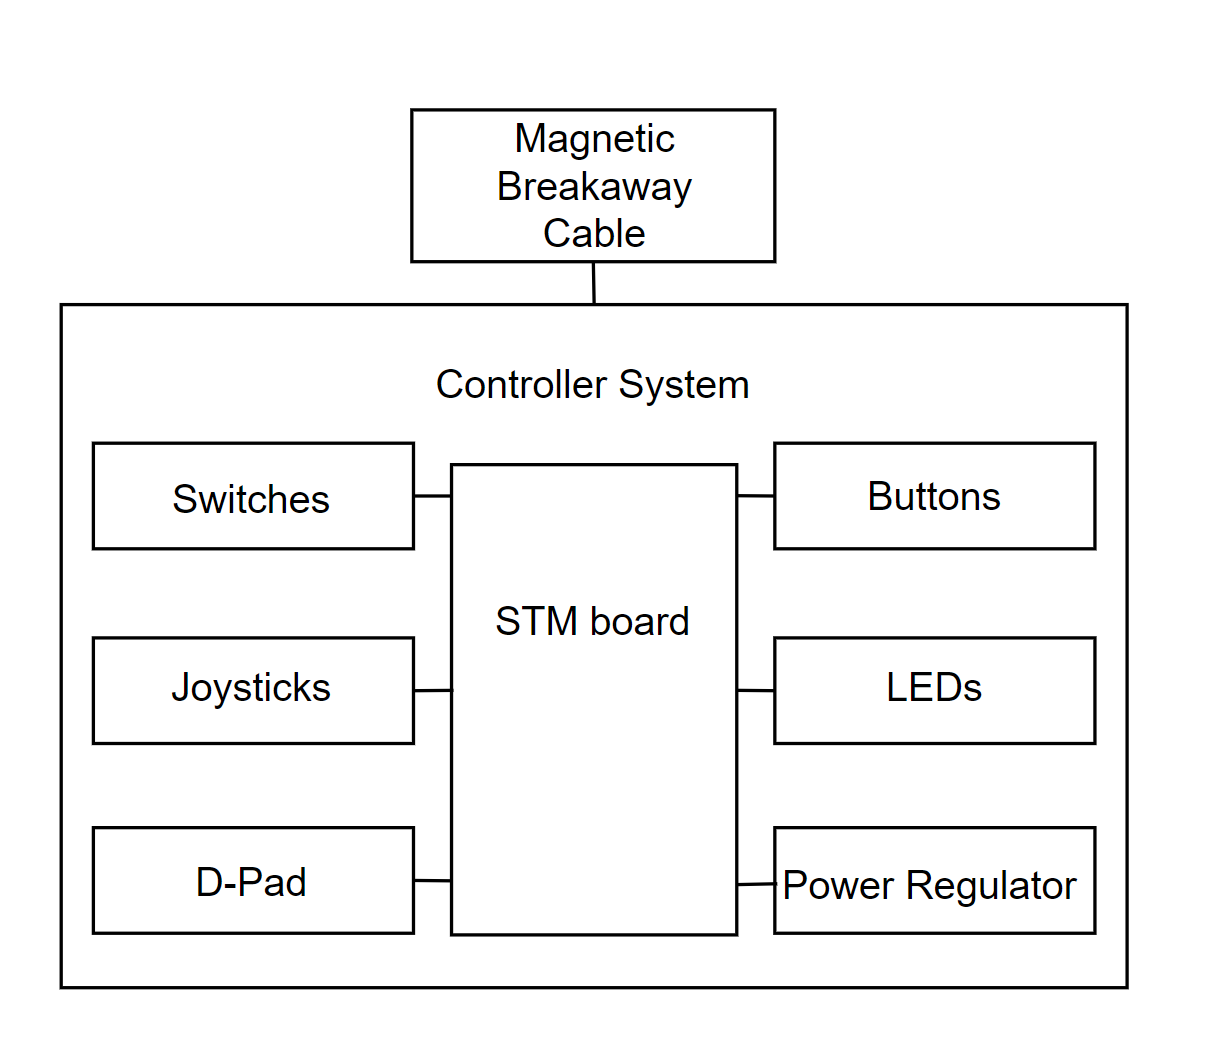
\includegraphics[width = 8cm]{MagneticBreakaway.png}
    \caption{Controller Hardware Diagram}
\end{figure}

\textbf{Results Indicative of Successfully Completed Stage}\\
1.	Motors respond to user inputs from the controller\\
2.	The breakaway cable's functions work as intended\\
3.	Motors are immobilised when the breakaway cable is disconnected\\


\subsubsection{Stage 3}

Duration: 2 weeks

\textbf{Assemble a Chassis}\\
Create a chassis out of aluminium extrusion that abides by legislation for mobility scooters and will fit underneath EVs with a ground clearance of 155mm.

\begin{figure}[h]
    \centering
    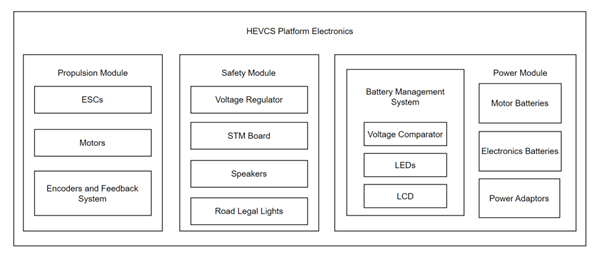
\includegraphics[width = 8cm]{PlatformHardware.png}
    \caption{HEVCS Platform Hardware Diagram}
\end{figure}

\textbf{Power System Integration}\\
The motors and power systems are mounted to the chassis, and the platform’s ability to be navigated by a user with the remote is trialled in a closed environment.

\textbf{Results Indicative of Successfully Completed Stage}\\
1.	A chassis with a high standard of structural integrity \\
2.	The maximum height of the platform is under 150mm\\
3.	The chassis and motors are combined to create a mobile platform\\
4.	The user inputs on the controller perform the correct functions\\
5.	The platform is mobile and can travel on flat surfaces\\

\subsubsection{Stage 4}
Duration: 3 weeks

\textbf{Weight Bearing Chassis}\\
The chassis is upgraded to support the weight of the payload, a 100kg battery, without compromising functionality.

\textbf{Battery Management System}\\
All electronic equipment necessary to display the current capacity of the platforms power and the charging battery's power are installed.

\textbf{Results Indicative of Successfully Completed Stage}\\
1.	The chassis rigidity is sufficient\\
2.	The chassis can transport the required payload on various terrains\\
3.	The system power system can be charged and monitored\\
4.	The payload battery can be charged and monitored\\

\subsubsection{Stage 5}

Duration: 2 weeks

\textbf{Object Avoidance}\\
The LiDAR system will be implemented to incorporate object sensing and ranging into the user assisting features.

\textbf{Step and Incline Management System}\\
Software implemented to immobilise the motors when the user attempts to drive the platform up or down a set of three or more steps or an incline of more than 20 degrees. The calculations for these boundaries have been calculated and documented in the project’s OneNote.

\textbf{Lights and Alarms}\\
The installation of a lighting system that abides by the relevant laws, detailed in the relevant legislation section, for a class 2 mobility scooter.

\textbf{Results Indicative of Successfully Completed Stage}\\
1.	Relevant vehicle legislative requirements are met\\
2.	The LiDAR can detect objects within a specified distance and highlight them as a potential hazard\\
3.	When hazards are identified, the platform will enter an immobilised state and override the user’s input if a collision is going to occur\\
4.	The system will not attempt to traverse inclines/declines greater than 20 degrees\\
5.	The platform can determine the appropriate drop it can attempt to traverse, with the maximum drop being defined as three steps\\

\section{Team Organisation}\label{sec:Team_Organisation}

\subsection{Tasking}\label{sec:Tasking}

The tasking is delegated on a Kanban board, with a description of the planned action items and a completion deadline. As the project had an industrial sponsor, this task log was used to implement additional requirements. These focused more on the who, what, and why questions that arose from collaborating directly with a customer. The incorporation of the Kanban board into the Microsoft Teams enabled notifications and reminders for task deadlines and increased the efficiency due to being inside of the Teams channel.

\subsection{Leadership and Team Organisation}\label{sec:Leadership_and_Team_Organisation}

The leadership approach used in this project is democratic, drawing upon individual’s knowledge and skills in relation to decisions. Democracy ensures that all four members are heard as equals, with the role of the leader within the group alternating when meetings are held. This method has benefited the project by allowing each member to influence the operational style of meetings, providing an opportunity to explore alternative methods of delivery. Elements of affiliative leadership have been utilised to focus on building relationships and facilitating communication. An example if this refers to a situation where illness affected the performance of a member, and upon returning to work they required an additional meeting to reintroduce themselves back into their role. The purpose of this meeting was to discuss the week’s progress, understand the decisions that had been made during the absence and facilitate their incorporation back into the team’s changed environment.

\subsection{Team Member Roles and Responsibilities}\label{sec:Team_Member_Roles_and_Responsibilities}

\begin{figure}[H]
\centerline{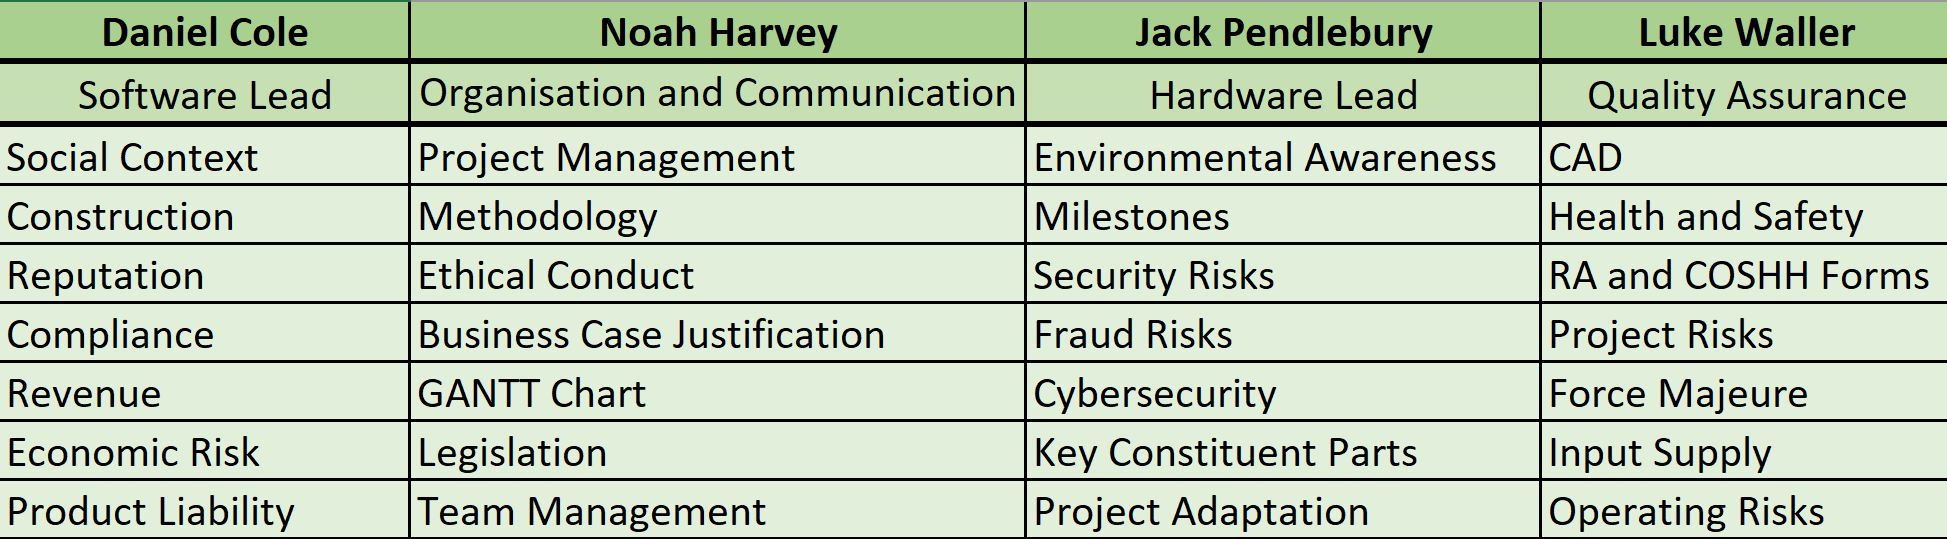
\includegraphics[width=1\textwidth]{TeamRoles.png}}
\caption{Team member roles and responsibilities}
\label{fig:figure_1}
\end{figure}

\textbf{Jo Byrne} is the employer engagement supervisor and the manager for the ESF Smart Specialisation project. Her role within this project is to facilitate liaison between Sirmon and the sponsorship scheme to ensure that, as a customer, Sirmon are satisfied with the performance of HEVCS. Jo attends and schedules regular meetings with the team and Sirmon both together and individually.
\\
\textbf{Jake Gibson Shaw-Sutton} is the project supervisor who attends meetings with the immediate project team and with Sirmon Industries.
\\
\textbf{Paul Davey} is the module lead, requiring project overview meetings monthly. He holds the authority to approve health and safety risk assessments, COSHH forms and access to the project budget.
\\
\textbf{Sirmon Industries}, consisting of Heather and James Sirmon, are the sponsors of the HEVCS project. The specification was written with their requirements for the product, and so they have a higher level of influence in the project and the tasking. The development cycles, stage boundaries and milestones were written in accordance with the scope the team defined during meetings with Jake and Jo.

\subsection{Meeting Structure}\label{sec:Meeting_Structure}

Another main principle of the agile methodology used is that the customer and developers work together daily throughout the project. The team will meet every Tuesday and Friday to discuss the tasking and research development for individual members. Involvement from the customer is paramount, with all advances within the project's operations reported and made accessible on the team's channel. Advantages of regular contact include the minimisation of confusion, specifications, and the incorporation of everybody's goals.
\\
With face-to-face conversation being the most efficient way of discussing the project, the team meet weekly with the customer on Zoom or in person. Conversing in this manner benefits the customer as they can bear witness to the achievements and provide feedback instantly. Additionally, emails are used to transfer documents for review and discussion, and group chats enable instant messages to be received. For this project, the group chat has been vital for planning, acknowledgement of receipt of documents and daily updates. The digital record of communication also provides accountability for both parties, in the event of a dispute.
\\
Project related research will be carried out throughout the week, with write ups and findings being reported to the entire team every Monday morning. This way, any problems, such as incomplete tasks or actions from previous meetings, have been highlighted and discussed at the start of the working week. Tuesday afternoons will be used to facilitate group efforts to overcome problems and employ the tools and methods necessary.
\\
Bi-weekly meetings will be held with Sirmon Industries, our supervisor (Jake) and the employment engagement officer (Jo). These meetings are used to discuss project progress in detail to facilitate accomplishing both academic and industry criteria. In semester 2, these meetings with Sirmon will run every week.
\\
Fridays will allow the team to come together and reflect upon the week. All team members will provide an overview of their week, how they felt about the tasks they completed and how the team’s approach could be altered for the following week. This will involve confirming availability, especially as other aspects of the module begin to take precedence of the Tuesday afternoon timetabled sessions.

\section{Health and Safety}\label{sec:health_and_safety}
\subsection{Risk Assessment}\label{sec:risk_assessment}

A Risk Assessment has been conducted to critically evaluate the risks involved with the project's operation. This includes their severity, and the best way to mitigate them.
The Risk Assessment is a useful document for tracking and monitoring the risks of the project.
This document serves as a safe practises guide for operating dangerous tools and machinery.


For the Risk Assessment, refer to the separate document.

\subsection{COSHH Forms}\label{sec:coshh_forms}

A series of control of substances hazardous to health (COSHH) forms have been completed in accordance with manufacturers recommendations.
The COSHH forms outline the safe usage for substances that are potentially damaging to both the user's health and the environment.
These forms are a useful aid for tracking and monitoring the potentially harmful substances used within the project.
These documents serve as safe practise guides for working with dangerous substances.


For the COSHH forms, please refer to the separate documents.

\subsection{Saftey Measures}\label{sec:safety_measures}

Given the large form factor and heavy payload requirements of the HEVCS platform, following appropriate safety measures and protocols will be vital in ensuring the wellbeing of the team members.
Before beginning any hardware development, all participating members will be required to read the relevant risk assessments and COSHH forms for the activity they are undertaking.
This will ensure the safest possible working environment in which team members are aware of the risks of any given activity, and how to mitigate against them.
If these protocols are not followed it could lead to potentially life altering or fatal accidents.
As a result of this, multiple safety measures have been considered and implemented.
These have been outlined below.

\section{Comercial Risk Evaluation}\label{sec:Commercial_Risk}

\subsection{Security and Fraud}\label{sec:Security_and_Fraud}

Commercial Fraud is not a crime within itself in the eyes of English law, however there are numerous actions that can constitute fraud. These include but are not limited to fraudulent misrepresentation or deceit; conspiracy; inducing a breach of contract; bribery; certain breaches of fiduciary duty; breach of trust, for example dishonest assistance; and claims for wrongful or fraudulent trading under the Insolvency Act 1986\cite{Fraud_Intro}.
\\
Some examples of these actions are things such as the misappropriation of assets and funds and overstating expense and budgetary claims. These risk factors can be mitigated through thorough bookkeeping and holding team members accountable for purchases using the budget. Every purchase using the budget should be agreed upon unanimously before having the purchase order sent off for consideration. Each purchase order will additionally be verified at the other end, whether by the university stores or the company sponsor. This two-layer verification will stop any fraudulent behaviour – intentional or otherwise.
\\
Other types of fraud listed above are less applicable to the sponsor-student relationship that this project revolves around, and furthermore are covered within the University’s Student Charter. Breaches of this hold severe academic consequences, and the team members will be encouraged to report any potential breaches to the relevant parties, such as the project supervisors, module leaders, and faculty staff.
\\
Cybersecurity attacks continue to increase year-on-year, despite a growing reliance on technology and cloud-based solutions for common services\cite{Checkpoint}. 2022 saw a particularly large vulnerability exploited in the Apache web server software, as well as a significant increase in cyber-warfare attacks directed from within the Russo-Ukrainian conflict. This has only added to the increase in the number of attacks, and corporate entities everywhere are being encouraged to take further measures to secure their assets\cite{Forbes_Cyber_Stats}.
\\
By far the most common attack vector is through compromised account credentials. The project’s sensitive code will be stored in a private Git repository, and team members will be encouraged to take action to secure their own accounts with unique passwords and two-factor authentication. GitHub is considered secure, the largest breaches being due to authorisation tokens stolen at the company level, as opposed to server-side breaches.
\\
Similar precautions will be taken for OneDrive. OneDrive will function as a secure cloud storage location for project materials, such as risk assessments, execution plans, methodology reports, and other such materials. OneDrive shares the same vulnerabilities that GitHub does regarding the weakest link being the human layer. As previously stated, team members will be encouraged to use unique passwords, and access will only be given to team members and university staff on a need-to-know basis.
Materials graded confidential will never be shared beyond the team and relevant staff, and any public release of confidentially graded material must be authorised by the sponsor first. This release will be kept to the bare minimum, and any information within a document to be released that is not authorised will be redacted.

\subsection{Construction}\label{sec:Construction_Risk}

Construction risks are the risks to the construction phase of the project. These risks can range in type, from materials not arriving on time to components being damaged on arrived (DOA). These risks are easy to mitigate against using various methods. It is import for a project with such tight time resections that the components are not ordered using a just in time \cite{Just-In-Time_Manufacturing} manner. For a project of this nature, it is important that the materials are obtained well in advance of needing them just in case there are only issues that could cause a significant delay. This also ensures any issues with the components can be sorted well within the margins of safety of construction time for the project.
\\
Drying/Curing/Hardening times are also important to consider when evaluating the construction timeline for the project. It is important to evaluate this to make sure that time is not being spent waiting for assemblies to dry.
\\
Some instances of construction risks are outlined below:

\begin{itemize}
    \item Materials not arriving on time (being delayed)
    \item Damage to components and parts
    \item Delays in received machined/cut parts delaying construction
    \item Drying/curing/hardening times
\end{itemize}

\subsection{Compliance}\label{sec:Compliance_Risk}

When a company begins a project, they will have to make sure that they are complying with all relevant legislation. If regulations outlined within the legislation are not met, then there could be financial or legal penalties. To make sure that the HEVCS platform can be used on pavements, the team are making sure that it will keep to the legislation pertaining to class 2 mobility scooters. This legislation describes the max weight, dimensions, and the max speed that the platform can be. The team will also make sure that any batteries that they use will comply with the safety standards set in the UK. Legislation will be regularly consulted, and any adjustments made to keep the platform within the requirements. Product safety standards

\subsection{Revenue}\label{sec:Revenue_Risk}

Revenue can be affected by a range of risks, including operational, reputation, economic, competition and force majeure. If precautions haven’t been put into place for these risks, the revenue of the project may be negatively impacted. Each risk has been evaluated and steps to alleviate them have been put into place.
\\
Reputation of the company has the potential of impacting a project financially, either positively or negatively. Damages to reputation can come from actions that can be discourteous or incompetent. The main potential for this project to gain negative publicity will come from either: the team saying or posting something online which paints Sirmon Industries in a negative light, or the final product being built to poor standards. To prevent these issues, the team will be careful with what they post online or what they say to potential customers. making sure that they do not accidently create any adverse view towards Sirmon Industries. To make sure the HEVCS platform is made to the best quality possible, the team will extensively research each possible component and select based on quality and budget of the project.
\\
Competing companies could develop a product that encroaches on the HEVCS platform, decreasing the demand for it and potentially reducing the prospective revenue. Also, companies might already have a product that solves the same problem as the HEVCS platform. To make sure that this does not happen, the team have researched IPs to make sure that the HEVCS platform will not infringe on any other product.
\\
With the fluctuation of the market constantly affecting the economy, a project will be met with some economic risk. Currently, the UK is facing an economic crisis, with inflation being at a 30-year high and the country having entered a recession. To try and mitigate any risk that might arise from these economic changes, the team will keep approximately £500 of the budget in reserve, to absorb any potential cost fluctuations.
\\
Operating Risks are the risks resulting from ineffective or failed internal processes, systems, people, or external events that may cause disruption to the flow of business operations. These risks can be due to Employee error, criminal activity such as fraud, and even physical events. These can all trigger operational risks.
\\
Examples of Operating risks are outlined below:

\begin{itemize}
    \item Ineffective Communication between members of the team or between the project team and Sirmon Industries
    \item Not being able to afford the best components causing failures and setbacks within the project
    \item Inflation causing all components to become more expensive to purchase
    \item Scope creep
\end{itemize}

Construction risks are the risks to the construction phase of the project. These risks can range in type, from materials not arriving on time to components being damaged on arrived (DOA). These risks are easy to mitigate against using various methods. It is import for a project with such tight time resections that the components are not ordered using a just in time \cite{Just-In-Time_Manufacturing} manner. For a project of this nature, it is important that the materials are obtained well in advance of needing them just in case there are only issues that could cause a significant delay. This also ensures any issues with the components can be sorted well within the margins of safety of construction time for the project.
Drying/Curing/Hardening times are also important to consider when evaluating the construction timeline for the project. It is important to evaluate this to make sure that time is not being spent waiting for assemblies to dry.
Some instances of construction risks are outlined below:

\begin{itemize}
    \item Materials not arriving on time (being delayed)
    \item Damage to components and parts
    \item Delays in received machined/cut parts delaying construction
    \item Drying/curing/hardening times
\end{itemize}

\subsection{Project}\label{sec:Projcet_Risk}

Project risks outline any person/interpersonal issues that may arise during the project. These risks are hard to mitigate against and can happen at any point. Because these risks are unavoidable and unplanned, a contingency plan must be always in place just in case any issues may arise.
\\
Contingency plans include, moving meetings to an online format in case of unavailability of persons to attend meetings in person. Reschedule meetings for when all attendees are available. Understand the workloads of everyone within the team so if a member is unable to continue working for a certain time. This would allow other team members to reassign tasks accordingly.

\begin{itemize}
    \item Someone falls ill/gets covid
    \item Family emergencies
    \item Personal economic disaster (someone can no longer afford to study at university)
\end{itemize}

\subsection{Input Supply}\label{sec:Input_Supply_Risk}

Input Supply risks are risks involving the obtaining of materials and components that are needed for the project. It encapsulates the sourcing and arrival of components and how this may affect the progress made on a project. In the current economic climate supply chains have been drastically affected; they are unable to continue to supply the needed number of components. Due to the high demand and short supply, components are becoming more expensive and more difficult to obtain. The supply shortage has many contributing factors such as, the worldwide silicone shortage, the COVID-19 pandemic, and the on-going war in Ukraine.
\\
Although parts of supply chains are beginning to see a return towards normality, there are still major disruptions on many services which are estimated to continue until, at least, 2023/24. Therefore, this will be a consideration for the whole duration of this project and will need to be continually monitored.
\\
A few examples of Input supply issues are listed below:

\begin{itemize}
    \item Components becoming unavailable due to demand issues
    \item Shortage of required components need for construction
    \item Long lead times on components due to various influencing global factors
    \item Only look at things available within the UK (United Kingdom) to save time and money
\end{itemize}

\subsection{Operating}\label{sec:Operating_Risk}

Scope creep, otherwise known as requirement creep, or feature creep, refers to the tendency for a project’s requirements to bloat overtime, with superfluous requirements added as the project progresses. Scope creep can negatively affect a project in several ways. Adding additional requirements beyond what the project was originally specified dilutes the talent pool available, reducing the overall quality of the final product.
\\
Customer requirements can change through a project’s development, and this does not always constitute scope creep. Creep is characterised by the uncontrolled changing of requirements in a manner that is not conducive to development goals.
Scope creep can be caused by several factors. A lack of detail within the project requirements and goals can leave project direction up for interpretation. This gives an avenue for scope creep to be introduced. The scope should be clearly defined and strongly controlled, ensuring all parties agree on the direction of development.
\\
Weak leadership can also cause scope creep. It is the project manager’s responsibility to evaluate stakeholder requests and deny any that inflate scope creep unnecessarily. All communication with stakeholders should be strong and clear, to lower the chance of miscommunication. This is especially important in regard to discussing project goals and specification.
\\
Stakeholder’s may also be a direct cause of scope creep. While stakeholders may agree on the final objective of the project, there may be differing opinions on project priorities. These differing priorities may lead to stakeholders pushing the project in alternative directions, spreading development resources thin. This is another reason as to why strong communication is vital, and good leadership can prevent stakeholder misconceptions from altering the project strategy.
\\
The most serious form of scope creep can be introduced by not taking advantage of user feedback. If end user’s feedback is only considered at the end of the development cycle, with no time designated to account for changes introduced by this feedback, a project’s final stages can be derailed by said feedback. User testing feedback should be focused on to the appropriate areas, to avoid scope creep and allow for as focussed a final development period as possible.
\\
Avoiding scope creep is an involved process, which begins from the beginning of development and continues throughout. Once the specification is created, it is important to check that all parties are clear on the details and overall direction of the project. Throughout development Variance Analysis will be performed, comparing the current project progress to the original specification. Each identified deviance will be investigated, and the cause and magnitude found. Based upon this information, a cause of action will be decided. Preventative or corrective actions can be taken to restore project direction and alleviate divergent project direction. Each change requested, as well as its associated course of action, will be added to the execution plan.


\section{Ethical Conduct}\label{sec:ethics}
\subsection{IET Rules of Conduct}\label{sec:IET_rules_of_conduct}
The IET have provided guidance to support its members in taking responsibility for their decisions and acting in an ethical manner. The Rules of Conduct \cite{Rules_of_Conduct}, written in accordance with Byelaw 31, are used to aid individuals in meeting professional standards and principles adopted in the engineering industry. By joining the IET, all the team members working on this project have made a commitment to take an ethical stance that considers society, the environment, and the requirements of the employer. In addition to this each individual should manage conflicting interests from team members, the university and sponsor with integrity. With this project being sponsored and conducted within a university, all members have a duty to uphold the reputation and standards of Sirmon Industries and the University of Plymouth.

\subsection{Ethical Principles - Engineering Council}\label{sec:ethical_principles_engc}

The Engineering Council and the Royal Academy of Engineering produced a Statement of Ethical Principles that details the four ethical principles that engineers must follow to maintain and enhance the wellbeing of society. It is a requirement that IET members observe and enforce these principles to uphold the reputation of the organisation.

\subsubsection{Honesty and Integrity}

All members must remain honest, fair, trustworthy, and open to discussion. The team must act responsibly and consider how their actions as individuals affect others, especially the reputation of Sirmon and the university. The project itself is confidential and all information related to the project
should be treated as such.

\subsubsection{Respect for Life, Law, Public Good and The Environment}

The platform must obey all applicable laws and regulations, along with the acknowledgement of physical, cyber and data security. The project itself sets out to overcome obstacles that the public encounter when they wish to use an EV but have no access to a charging point. By developing such a solution, the quality of the natural environment is increased by decreasing the number of traditional fuel ran vehicles on the road.

\subsubsection{Accuracy and Rigour}

All individuals within the group acknowledge the duty of care required to complete such a project. It is essential that all tasks are conducted by those who have adequate knowledge and technical understanding of the skills required. Additionally, risk assessments must be completed before the equipment and components are acquired. This is to ensure that risks have been identified, managed, and mitigated.

\subsubsection{Leadership and Communication}

All stakeholders must be made aware of the current tasking of the project through various forms of communication. Regular meetings must be held and used to raise concerns and plan the next tasks. The group itself does not contain a leader as all members operate as equals, promoting equality and inclusion. Every individual involved in the project and its various aspects must promote honesty and respect. This approach is also encouraged when challenging statements and concerns to remain professional.


\subsection{University of Plymouth's Research Ethics}

As the HEVCS platform is not storing data, or putting names to any data that may collected, the Research Ethics are not breached and therefore do not need to be evaluated for this project \cite{Research_Ethics}.

\subsection{Application of Ethical Conduct}
Engineer’s must limit any danger of injury or damage to the environment, including private and public property. To mitigate the risk of either occurring, the platform will only operate when the owner is physically tethered to the system via wired controller. There will be sensors used to cut off power to the motors when obstacles (be it objects or humans) are in the way. There will be security measures in place to unlock the platform from its stored state, with further implementations to ensure that.

The platform will not obstruct public pathways, as it will be stowed underneath the car or on the user’s property. The user has the responsibility to safely secure the platform within their home while it charges or locked to their car. If the device is not in use, it will be stored inside their home. If there is an obstruction preventing the user from placing their charging platform underneath their car, or within the vicinity of their own parking space – they must make the informed decision that it is not safe to charge their vehicle.

The way in which the platform is manoeuvred for storage will use the drive train to aid with lifting the system into place. This will ensure it is accessible to disabled people and the elderly. The mounting station in which the platform will be stowed in while engineers would install charging, in the same manner that EV charging ports are installed into the user’s home. The due diligence regarding safe placement of the station, power limitations and other safety factors will be conducted by the installation engineer.
The use of a LiDAR could be cause for concern if the data from the sensor is being utilised for anything other than object avoidance. That data could be used to create a map of the user’s home, which could a breach in security. As the LiDAR sensors are only used in a reactionary capacity, none of the data from the sensors is being stored and therefor is not accessible outside of the system. This negates the privacy concern of using these sensors for the project.

\section{Product Saftey and Liability}\label{sec:Product_Safety_and_Liability}

\subsection{Consumer Protection Act 1987}\label{sec:Consumer_Protection_Act}

The Consumer Protection Act (CPA) holds manufactures accountable for the goods they produce. Products include goods, components or the raw materials used. Getting injured by a defective product would entitle anyone to compensation, not just the consumer. For a product to be considered defective, the safety of the product is not at a standard a person would expect \cite{Consumer_Protection}. A claim can be made if a defective product has caused a death, injury, or private property damage equating to £275 or more.
\\
Since the HEVCS platform will be a prototype, there is not a concern with the complying with the CPA. However, the platform will be tested at every step of development to guarantee that there are no defects present.

\subsection{Product Warranty}\label{sec:Product_Warranty}

A warranty gives reassurance to the customers that the purchased product will perform as the manufacture intended and defines what compensation will be provided if it does not. \cite{Warranty} A warranty can have exceptions with them such as an expiry date, or the product not being used as intended. There are two types of warranty implied and expressed. Implied warranty comes with almost any consumer product, and it guarantees that the product will work as intended. An expressed warranty is given by the manufacture describing the specifications that the product will work to, and if it does not, the manufacturer will replace or repair the product. \cite{Warranty}
Due to the HEVCS platform being a prototype, a warranty will not be a concern. A company selling the product will have to put this into consideration. The warranty would be broken if the users were to try and modify the platform in any way. Also, the platform will have to be controlled with the intended controller, if another controller were to be used this would constitute a bypass of safety protocols. Any required repair or replacement would be charged to the customers.

\subsection{Accident and Injury Liability}\label{sec:Accident_and_Injury_Liabilty}

Product Liability Insurance is cover for a business that sells or manufactures products. It is rarely sold on its own but comes as part of a public liability insurance policy. Product liability insurance protects the business should a customer incur damages because of a fault with the product that the company has provided them. \cite{Liabilty_Insurance}  As we are not selling this product as part of this of this project, it is not an important consideration whilst making the HEVCS platform prototype. This will be a concern of any company that wishes to bring this product to market and sell it.

\subsection{Operational Safety and Compliance}\label{sec:Operational_Safety_and_Compliance}

Operational safety is when there are no unreasonable risks of injury or harm to a human due to defects, environmental conditions, or foreseeable misuse of the product. Product compliance means that the product meets the relevant legislation.
The HEVCS platform will have systems in place to stop the user from driving it into obstacles, potentially damaging it or a human. Limits will also be in place so that the user cannot make the platform traverse a slope which is greater than 20\% or climb more than 3 steps. If the controller disconnects from the platform, it will lock into place so that it won’t move until the controller is reconnected. Class 2 mobility legislation will be complied with so that it will be able to be used on pavements. While the HEVCS platform is a prototype, later developments the platform will need to be waterproof so that it can be used in wet conditions. \cite{IP_Rating}

\subsection{Intended Use and Relevant Safety}\label{sec:Intended_Use_and_Relevant_Safety}

Intended use is an important part of any instructional manual. It is a clear description of the products intended use of the product of machinery. It is a description that a company must treat very carefully as it sets the liability of the company and affects the further contents of the instruction manual. \cite{Intended_Use}
The intended use of this system is to transport the batteries from the user’s home to their EV and charge it. Any uses that do not fit under this description are deemed to not be intended use and therefore the manufacturer cannot be held responsible for any injuries incurred as a direct result of the HEVCS’ misuse. The provider of the HEVCS can be prosecuted only if the injury is as a direct result of the platform malfunctioning.
\\
The user of the HEVCS platform is not permitted to take the platform apart whether to replace components or perform maintenance. Further to this, to reduce risk of damage to the HEVCS platform, only suitable chargers will be able to be used for charging and operation of the platform.


\section{Environmental Analysis}
\subsection{Electric Vehicles}
Electric vehicles are widely toted to be a ‘green’ replacement for vehicles powered by traditional internal-combustion engines. There are, however, environmental concerns at all stages of an EVs lifecycle, which need to be carefully considered by any project seeking to use or benefit EVs.

The most effective way of comparing vehicle drivetrains on an emissions basis is by measuring the well-to-wheel (WtW) emissions\cite{Well_To_Wheel}. WtW represents a holistic way of comparing drivetrains, by considering the emissions from extraction to consumption. This is a combination of two other measures, well-to-tank (WtT), and tank-to-wheel (TtW). These are the extraction/generation, and the consumption measures, respectively.

 Battery Electric Vehicles (BEVs) emit no TtW emissions, as their electric drivetrain generates no greenhouse gases, however the WtT emissions are over double that of conventional ICE fuels. Even taking this into account, BEVs emit almost three times less CO2 into the atmosphere when compared to conventional ICE fuels. Petrol-powered plug-in hybrids (PHEVs) exist as a middle ground between BEVs and ICE engines, with even higher WtT emissions than BEVs, but WtT emissions are reduced to a third of petrol emissions and 2.5 times lower than diesel. Combined, this puts them between the two drivetrains for total WtT emissions.

It should be noted, however, that as of the time of this report, the UK’s energy mix was comprised of significantly higher amounts of energy generated using renewables instead of petroleum products or natural gas. Compared to the EU’s 17\% in 2020\cite{Energy}, the UK is currently generating approx. 45\% of its energy using renewables \cite{Electricity_Generation}. In practice, this would significantly lower the WtT cost of BEV and PHEVs to a point where it would be almost comparable with conventional fuels.

Another benefit of EVs is that these emissions are confined to the source, and so efforts to reduce the CO2/KG emitted can be concentrated on cleaner power generation, or better carbon trapping. An implementation that reduced emissions on EVs would have to be rolled out across an entire production run. Additionally, any EVs already on the road would not benefit from the greener technology unless a manufacturer issued a recall to perform upgrades, an expensive prospect. Given that the largest recall in history was twenty-one million vehicles by Ford in 1980\cite{Ford_Transmission}, and that in 2022 there are already sixteen million EVs\cite{EV_on_Road} on the road worldwide, a large-scale recall could quickly become infeasible.

\subsection{Battery Production}
One of the biggest environmental issues surrounding EVs is in the production of the batteries that power them. Modern battery technology relies on several rare-earth elements, most importantly lithium and cobalt\cite{Lithium_Source}\cite{Earth_Metals}. Lithium extraction has several devastating effects on the environment, effects further exacerbated by the environments that lithium is extracted in\cite{Lithium_Producers}. Lithium extraction is primarily done through the process of evaporation, where subsurface lithium deposits are driven to the surface by pumping water underground\cite{Lithium_Industry}. This water forms a salty brine on the surface, which is then left to evaporate for a prolonged period of time. Lithium carbonate is extracted from the distilled remains of the evaporation process, and this is processed into lithium-based batteries. Over two million litres of water are used per tonne of lithium extracted. Over half the water in Chili’s Atacama Desert is used for lithium extraction, depriving local communities and environments.

There are alternative methods of lithium extraction, but these have equally devastating effects on the environment. Open pit mining has been widely campaigned against for causing irrevocable harm to local environments and producing substantial amounts of heavy metal-based dust, which is toxic to humans\cite{Open_Pit_Mining}.

Lithium is also a finite resource, with current estimates placing the global supply of lithium at two hundred years’ worth. However, this will go down as production of EVs increases, assuming no non-lithium-based battery technology is adopted\cite{Not_Enough_Lithium}.

A large amount of research and development is going into alternative battery compositions, however lithium-based ones still remain the most cost effective for the energy density received and are the most widely available on the second-hand market.

Battery recycling has made great strides in recent years. A new Volkswagen site in Salzgitter aims to recycle five battery systems per shift, with an annual throughput of 3,600 battery systems for a total output of 1,500 tonnes of recycled material\cite{VW_Press_Release}. Initial expectations are to recover \(>\)70\% of the battery's constituent components by weight, with a target value of \(>\)97\% . Recycling EV batteries to augment global lithium supply would help to offset the increasing demand from the growing fleets of EVs.

EV battery capacity, represented as state of health (SOH), decreases through the lifetime of the battery in a linear manner that falls rapidly as it approaches end-of-life. This loss averages out to ~2.3\% per year, with the actual rate of SOH decrease affected by both usage and environmental factors\cite{EV_Battery_Health}. Typical EV battery warranties will last for eight years, leading to a source of batteries with a SOH value of ~80\%\cite{EV_Battery_Longevity}. These reduced capacity batteries are unsuitable for automotive purposes but have potential applications in use-cases that require less arduous capacity requirements.

\subsection{Chassis Manufacture}
Aluminium extrusion will be used to produce the prototype chassis. Aluminium is mined as bauxite ore, which is refined into alumina, from which aluminium is produced. However, the manufacture of aluminium extrusion is, compared to some other metal products, environmentally friendly. Over 75\% of the aluminium produced since 1888 is still in use today, and over 90\% of the energy used in European aluminium smelting is from zero-carbon sources.

The production of primary aluminium, that is, aluminium produced directly from alumina, has steadily decreased in its environmental impact. In 1995, producing one tonne of aluminium produced 16.5 tonnes of C02 equivalent. Updated processes dropped that to 12 tonnes of CO2 equivalent in 2018, and as of 2022, multiple aluminium producers have product available with a CO2 equivalent of less than 4 tonnes available\cite{Al_Manufac}.

By using aluminium instead of comparative materials such as steel, HEVCS hopes to lower its environmental impact. Once the prototype is no longer needed, the chassis can be disassembled to be recycled, with pieces of extrusion either re-used for other purposes, or sent to be recycled and re-made into new aluminium products.


Safety measures involve collision avoidance by using LiDAR sensors that detect obstacles around the platform, activating the brakes before impact.
The motors will also be stopped if the platform is trying to be driven down a slope greater than 20 degrees or a set of steps with a larger  than specified appropriate drop.
Thresholds will be set to stop the platform from traversing terrain it is not capable of.


The controller for the platform will utilise a breakaway connector which disconnects from the platform when it moves too far from the operator, causing the platform to halt operation, immobilising the motors.
The platform will also enter an immobilised state of operation if the controller becomes unresponsive at any point.


When testing the platform, a safe environment will be utilised. Only persons required to be in attendance will be allowed within the testing environment.
For full scale testing of a new firmware version uploaded to the platform, only the team members are allowed to be within the testing environment.
For finalised testing, the platform will be subjected to all environments that it is likely to experience in daily use, such as dark roads and uneven flooring.


To reduce the risk of a bug in firmware being uploaded to the full-scale platform, a series of small-scale mock-ups and testing rigs will be made and utilised.


Safe coding practises will be observed when writing and uploading code onto the platform.
These include changes to the code being checked, and a testing procedure being run before approval to upload the code is given.
This will implement a three-step code approval process starting with a test bench, continued into a small-scale model before being uploaded onto the full-sized platform.
Before changes to the code are uploaded onto the full-sized platform, the changes must be reviewed and approved by another member of the group.


Any safety critical sections of code will require the previously outlined levels of approval with further safety measures being implemented.
The safety critical code must be checked and approved by all members of the group.
This will involve a full review by the team including an outline of the changes presented by the group member who implemented them.
Safety critical elements of the code are defined as any code that modifies the locomotion of the platform or adapts how the platform behaves when the controller is disconnected.

\section{Social Context}\label{sec:Social_Context}

The HEVCS platform will be able to provide a service that many people can benefit from. With UK legislation banning the sale of new petrol and diesel cars in 2030, better infrastructure needs to be in place for charging EVs, otherwise they will not be an option for many people.
\\
While people living in rural areas more commonly have some form of off-street parking, many people within cities can only park on the street. Without a driveway charging points cannot be installed, increasing the difficulty of charging their EV. This leaves EV owners without dedicated parking few charging options. These include laying a large cable from their house to the vehicle or having to charge their car at a public charging point. An increase of EV owners will likely cause strain on the current charging infrastructure, making it difficult for people to get their vehicle charged. Also, having multiple homes running large cables across pavements will create a health and safety risk to pedestrians. The HEVCS platform will provide an option that reduce reliance on public infrastructure and stop people laying large cables out from their homes to their EV.  The HEVCS platform will be able to sit underneath the vehicle while charging it, keeping within the bounds of the vehicle, and not occupying any additional space.
\\
Another problem that the HEVCS platform could help solve is the issue of recovery when an EV has run out of charge. Instead of having to get the vehicle towed to the nearest charging point, the HEVCS platform can be taken to it and provide enough charge so that the vehicle can drive to a charging point.
\\
The HEVCS platform may also see use within a hire system, such as Santander Cycles. A docking station could be set up with multiple carriages, which the public would be able to hire. The HEVCS platform would allow for an EV charging infrastructure to be introduced onto a road without causing significant disruption to road surfaces or pavements.

\section{Internationalisation - Global Market}\label{sec:internationalisation}

Introducing the HEVCS to the global market is highly achievable but would need to be done with several considerations in mind.
Given the nature of charging batteries from within the home, suitable infrastructure would need to be evaluated.
Given that the UK runs off 230V 50Hz AC power, the HEVCS will be designed to run off these ratings.
This would work throughout Europe, due to the voltages being harmonised in 2003 (when the UK was still part of the European Union (EU))\cite{UK_Voltage_Change}, meaning that only the plug connected to the platform would need to be changed.
Using a universal plug connection, such as an IEC 60320, would allow the charging circuitry to be universal in any country that uses the same power levels as the UK.
Other locations, such as the United States of America (USA), use 120Vac so would require differing power circuit to be implemented\cite{Voltages_And_Frequencies}.


Along with charging circuitry, the HEVCS platform would need to be checked against the plurality of local legislation.
Local regulations for step height, doorframe size, and curb dimensions, would need to be checked and if required, the design may need to be adapted to accommodate global regulations.


The platforms classification may also need to be adapted, depending on the specific country requirements.
This could be anything from adapting the size of the platform, to reducing its payload.
Some of these may require a considerable redesign to accommodate regional legislation.
\newpage
\bibliographystyle{IEEEtranN}
\bibliography{refs}

\newpage
\appendix

\section{Car Dimensions}\label{app:Car_Dimensions}

\begin{figure}[H]
    \centerline{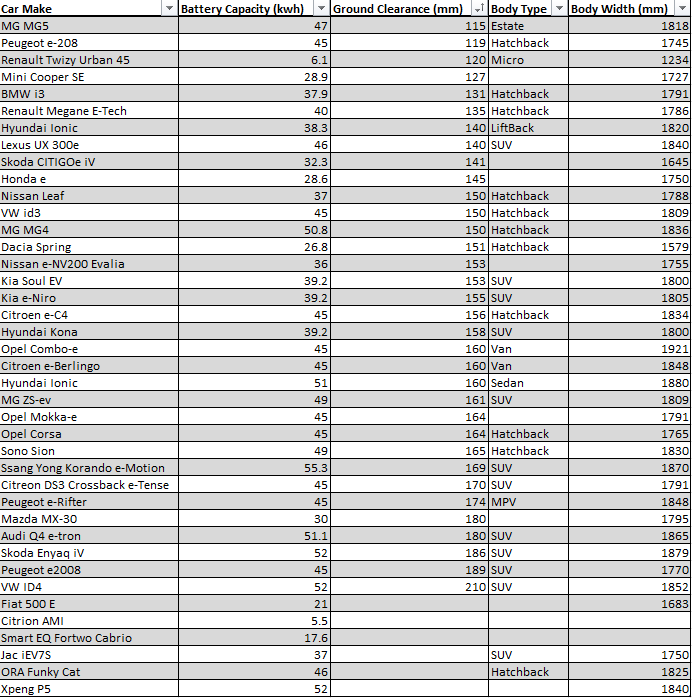
\includegraphics[width=1\textwidth]{CarDimensions.png}}
    \caption{Car dimensions research}
    \label{fig:CarDimensions}
\end{figure}

\section{Gantt Chart}\label{app:Gantt_Chart}

\begin{figure}[H]
    \centerline{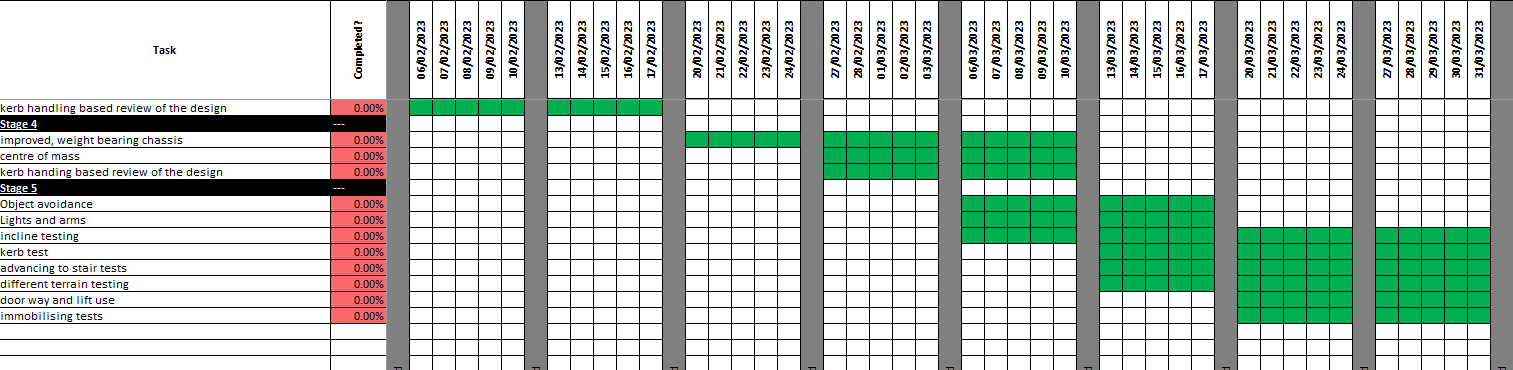
\includegraphics[width=1\textwidth]{GanttChart.png}}
    \caption{Gantt Chart}
    \label{fig:GanttChart}
\end{figure}


\end{document}